\documentclass[a4paper,11pt,dvipdfmx]{jsarticle}

\usepackage{bm}
\usepackage[dvipdfmx]{graphicx}
\usepackage[dvipdfmx]{color}
\usepackage{ascmac}
\usepackage{siunitx}
\usepackage{otf}
\pagestyle{plain}
\usepackage{float}
\usepackage[dvipdfmx]{hyperref}
\usepackage{pxjahyper}
\usepackage{here}
\usepackage{titlesec}
\titleformat*{\section}{\LARGE\bfseries}
\titleformat*{\subsection}{\normalsize\bfseries}
\usepackage{url}
\usepackage{docmute}
\hypersetup{% hyperrefオプションリスト
setpagesize=false,
 bookmarksnumbered=true,%
 bookmarksopen=true,%
 colorlinks=true,%
 linkcolor=blue,
 citecolor=blue,
}

% ↑ここまでいろんな設定


\begin{document}
%begin document から end documentの間のコードをコンパイルするようになってる

\section{\LARGE{導入(担当:田中)}}
基本的なルール\\
TeX上でのコマンドはバックスラッシュで始まるよ\\
beginなんちゃらで始まるやつは必ずendなんちゃらがいるよ\\
どんな見た目になるか見たいときは上のRecompileボタンを押す

\subsection{サブセクションのタイトル}
サブセクションだよ〜\\
スラッシュ2つで改行

1行以上開けると段落新しくなるよ

\subsubsection{サブサブ}
図の挿入\\

\begin{figure}[H]
\centering %中央揃え
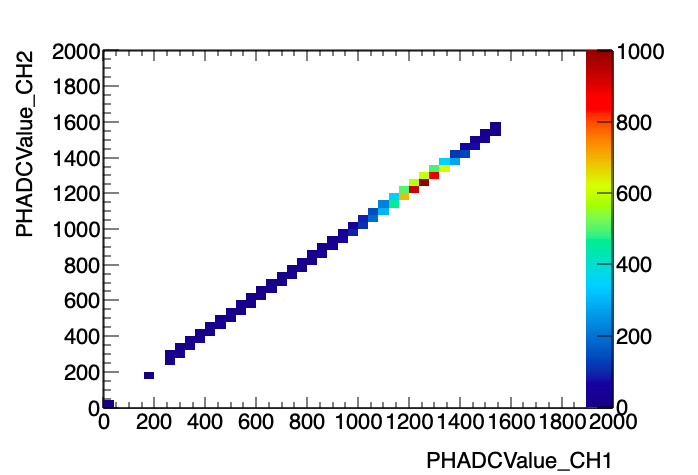
\includegraphics[width=100mm]{picture/daq/2ch2d.png} %widthで大きさの調整。{}の中は写真の居場所を書く。写真は左のpictureフォルダ内に入れてくだちい
\caption{図のタイトル} %タイトル
\label{2dhist} %2dhistという名前でラベル付する(後で引用したりできる)
\end{figure}

[図\ref{2dhist}]のように〜〜〜〜〜、、、、
これで引用できる

\newpage
これで新しいページ

ここから\\
\vspace*{10mm}\\
縦方向に10mmの隙間作れる\\



2つの写真を横並びに挿入する
\begin{figure}[H]
    \begin{tabular}{cc}
      \begin{minipage}[t]{0.45\hsize}
        \centering
        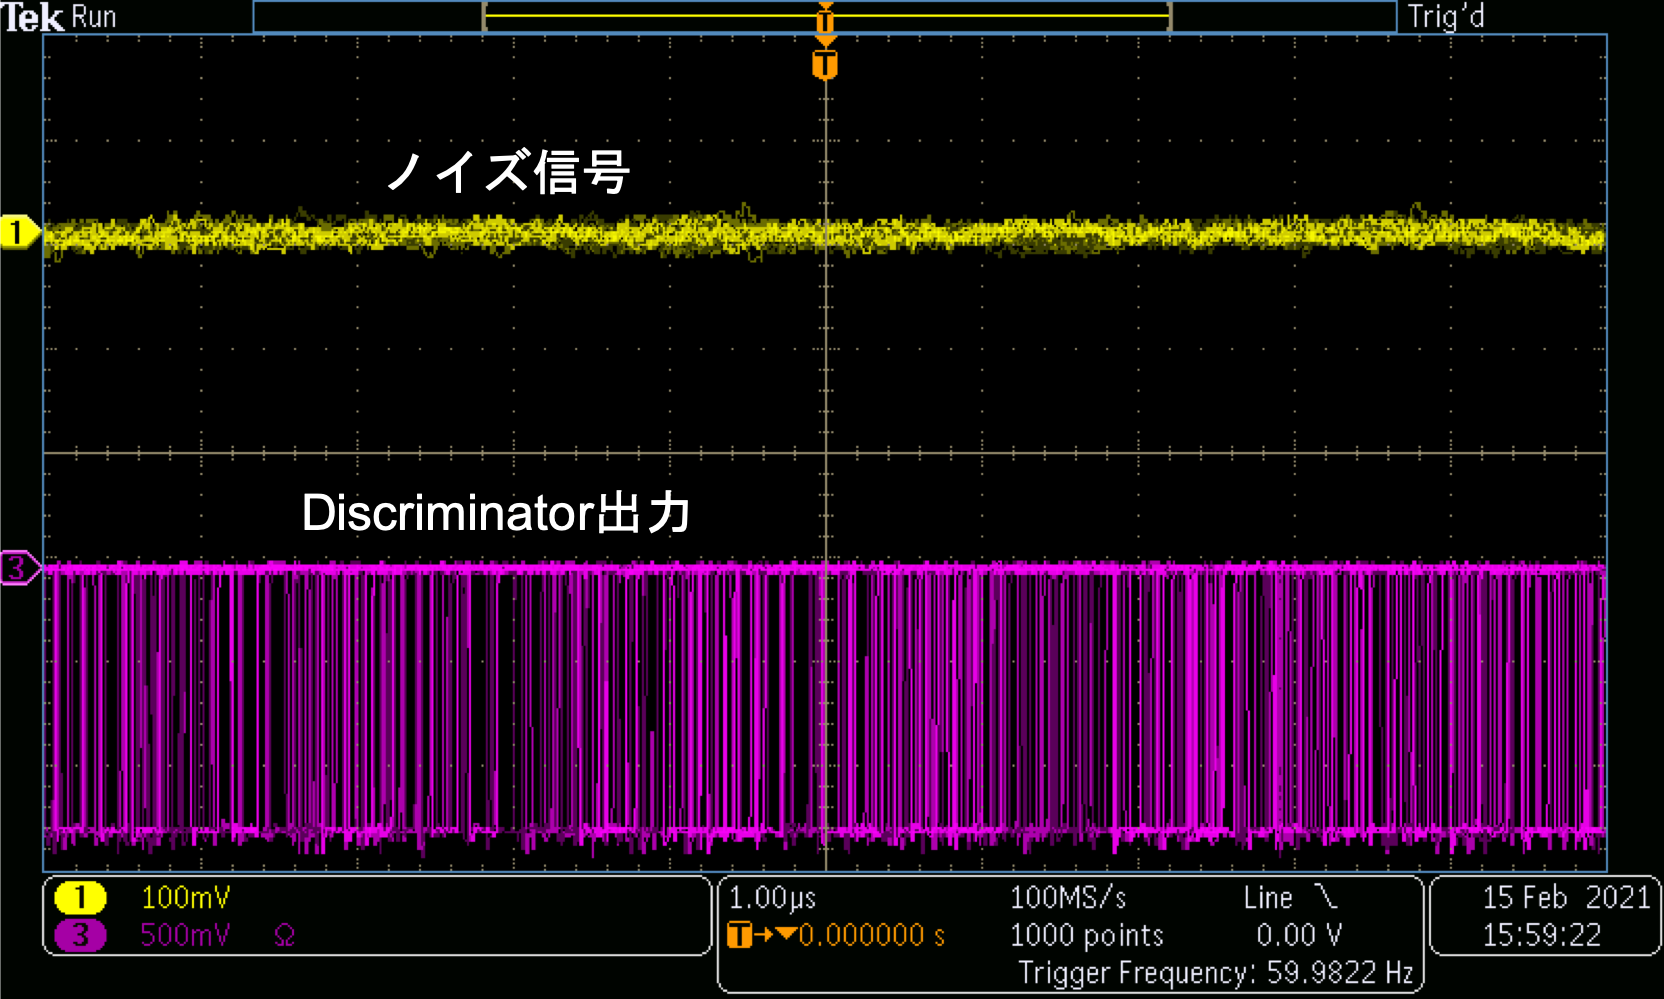
\includegraphics[width=60mm,height=42mm]{picture/daq/noise.png}
        \caption{ノイズ信号にディスクリミネーターが反応している様子}
        \label{noise}
      \end{minipage} &
      \begin{minipage}[t]{0.45\hsize}
        \centering
        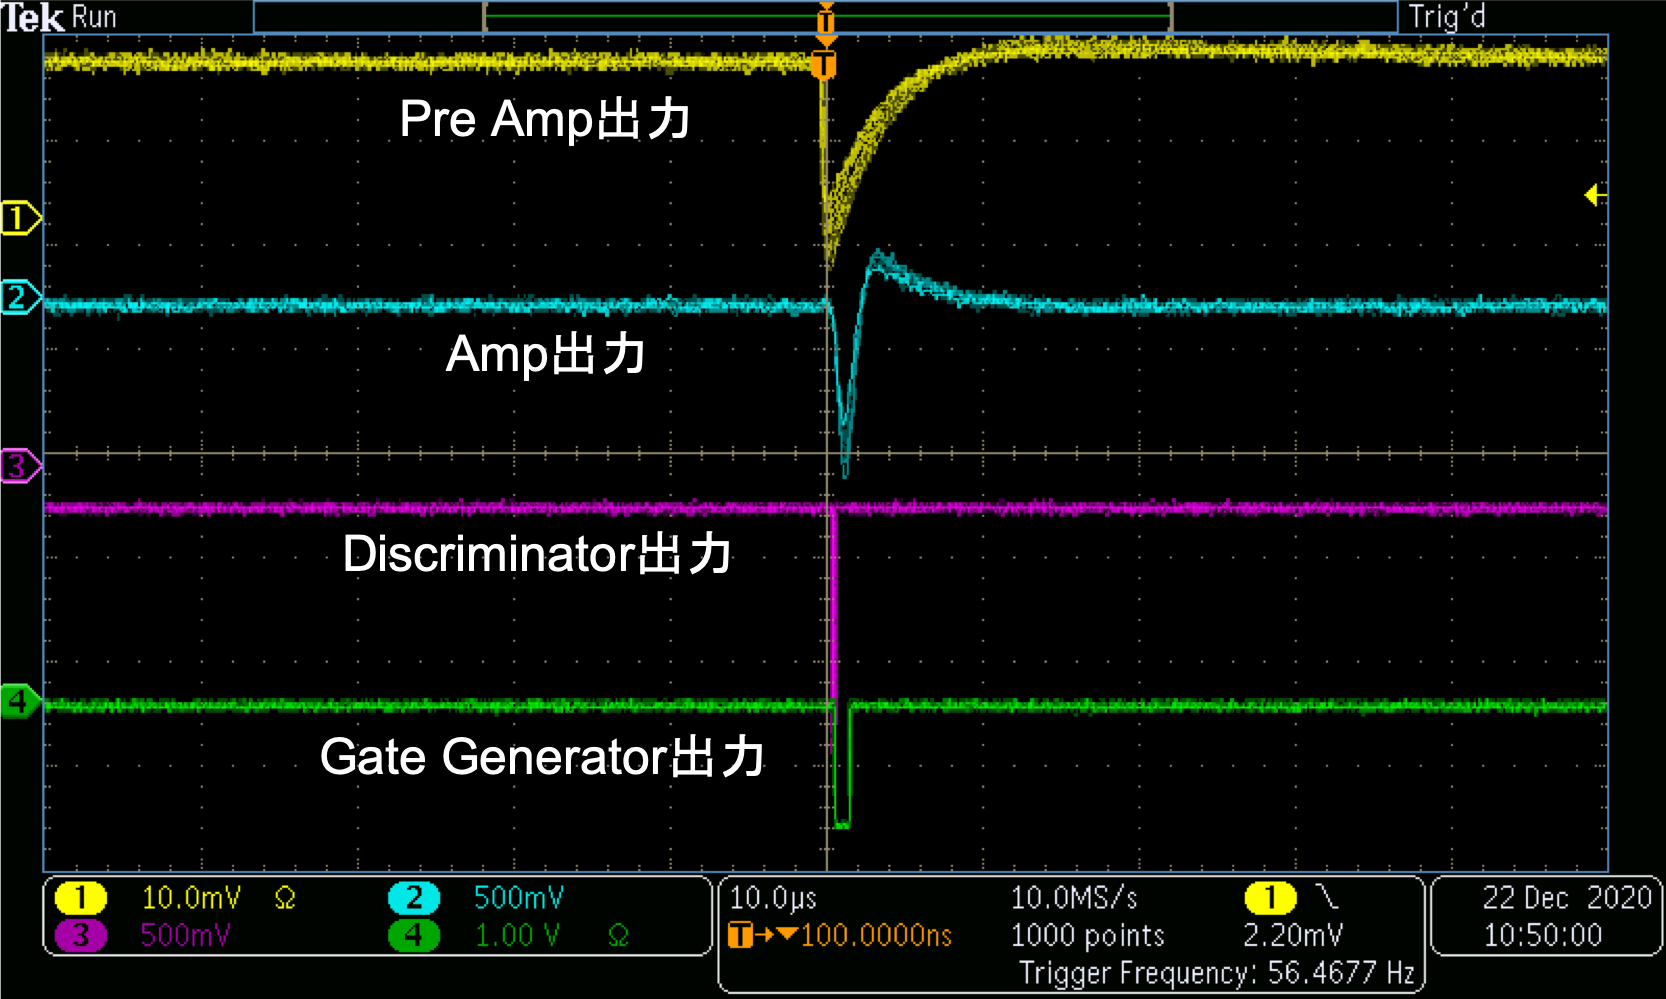
\includegraphics[width=60mm,height=42mm]{picture/daq/signal.png}
        \caption{適切な各モジュールの出力}
        \label{SiTCP2}
      \end{minipage}
    \end{tabular}
  \end{figure}



表を作りたいときは、\url{https://www.tablesgenerator.com}でWordみたいに打ってコピペするのが楽\\
例↓

\begin{table}[h]
   \caption{使用したVMEモジュール}
   \centering
   
  \begin{tabular}{ccc} \hline
  モジュール名 & 制作元:型番 & スペック等 \\ \hline \hline
  PHADC & 豊伸電子:8ch PHADC V006 & 
  \begin{tabular}{c}
    最大入力:4V\\
    逐次14bit変換\\
    入力インピーダンス:1k$\Omega$ \\
    最小Gate幅:500ns
   \end{tabular} \\ \hline
    SiTCP VME Master & BeeBeansTechnologies:BBT-002-2 &
    \begin{tabular}{c}
    通信プロトコル:TCP
   \end{tabular} \\ \hline

  \end{tabular}
  \centering
\end{table}

\newpage
\noindent %段落頭の1じ下げなし
数式を書くときは数式モードになってないとダメ。コマンドは地道に調べるべし\\
例えばべーてぶろっほ
\begin{equation}
\centering
\large
 -\frac{1}{\rho}\frac{dE}{dx} = \frac{4\pi{N_A}}{{m_e}c^2}{\left( \frac{e^2}{4\pi\varepsilon_0}\right)}^2\frac{Z}{A}\frac{1}{\beta^2}\left[\ln{\left(\frac{2m_ec^2\beta^2}{I(1-\beta^2)} \right)-\beta^2}\right]
  \label{BB}
\end{equation}

例えば文中に数式を入れたい場合は、$\alpha\neq\beta$のようにドルマークで囲めばOK\\


\LARGE{でかい文字}
\small{ちっちゃい文字} \\

箇条書き
\begin{itemize}
  \item 秋山
  \item 馬場\mbox{}\\
  こうするとここに書ける
  \item 山本
\end{itemize}

\end{document}